\documentclass[10pt]{article}
\usepackage[polish]{babel}
\usepackage[utf8]{inputenc}
\usepackage[T1]{fontenc}
\usepackage{graphicx}
\usepackage[export]{adjustbox}
\graphicspath{ {./images/} }
\usepackage{amsmath}
\usepackage{amsfonts}
\usepackage{amssymb}
\usepackage[version=4]{mhchem}
\usepackage{stmaryrd}
\usepackage{multirow}

\title{KOD }

\author{}
\date{}


\begin{document}
\maketitle
WYPEŁNIA ZDAJĄCY

PESEL\\
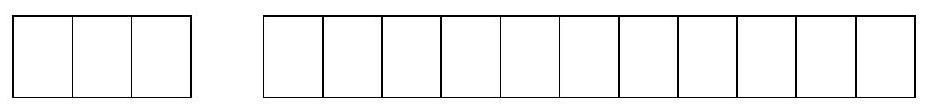
\includegraphics[max width=\textwidth, center]{2024_11_21_465acd0c12fa3e05e8a7g-01}

\section*{Miejsce na naklejkę.}
Sprawdź, czy kod na naklejce to E-100.\\
Jeżeli tak - przyklej naklejkę. Jeżeli nie - zgłoś to nauczycielowi.

\section*{EGZAMIN MATURALNY Z MATEMATYKI POZIOM PODSTAWOWY}
\section*{DATA: 5 maja 2022 r.}
GODZINA ROZPOCZECIA: 9:00 CZAS PRACY: \(\mathbf{1 7 0}\) minut LICZBA PUNKTÓW DO UZYSKANIA: 45

\section*{WYPEENIA ZESPÓŁ NADZORUJACY}
Uprawnienia zdającego do:\\
nieprzenoszenia zaznaczeń na kartę dostosowania zasad oceniania dostosowania w zw. z dyskalkulią.\\
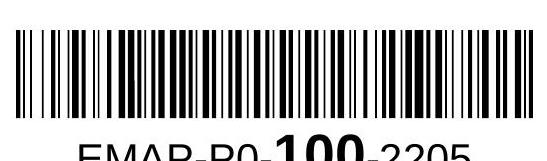
\includegraphics[max width=\textwidth, center]{2024_11_21_465acd0c12fa3e05e8a7g-01(1)}

EMAP-PO-100-2205

\section*{Instrukcja dla zdającego}
\begin{enumerate}
  \item Sprawdź, czy arkusz egzaminacyjny zawiera 25 stron (zadania 1-35).
\end{enumerate}

Ewentualny brak zgłoś przewodniczącemu zespołu nadzorującego egzamin.\\
2. Na tej stronie oraz na karcie odpowiedzi wpisz swój numer PESEL i przyklej naklejkę z kodem.\\
3. Nie wpisuj żadnych znaków w części przeznaczonej dla egzaminatora.\\
4. Rozwiązania zadań i odpowiedzi wpisuj w miejscu na to przeznaczonym.\\
5. Odpowiedzi do zadań zamkniętych (1-28) zaznacz na karcie odpowiedzi w części karty przeznaczonej dla zdajacego. Zamaluj \(\square\) pola do tego przeznaczone. Błędne zaznaczenie otocz kółkiem () i zaznacz właściwe.\\
6. Pamiętaj, że pominięcie argumentacji lub istotnych obliczeń w rozwiązaniu zadania otwartego (29-35) może spowodować, że za to rozwiązanie nie otrzymasz pełnej liczby punktów.\\
7. Pisz czytelnie i używaj tylko długopisu lub pióra z czarnym tuszem lub atramentem.\\
8. Nie używaj korektora, a błędne zapisy wyraźnie przekreśl.\\
9. Pamiętaj, że zapisy w brudnopisie nie będą oceniane.\\
10. Możesz korzystać z zestawu wzorów matematycznych, cyrkla i linijki oraz kalkulatora prostego.

W każdym z zadań od 1. do 28. wybierz i zaznacz na karcie odpowiedzi poprawną odpowiedź.

\section*{Zadanie 1. (0-1)}
Liczba \((2 \sqrt{8}-3 \sqrt{2})^{2}\) jest równa\\
A. 2\\
B. 1\\
C. 26\\
D. 14

\section*{Zadanie 2. (0-1)}
Dodatnie liczby \(x\) i \(y\) spełniają warunek \(2 x=3 y\). Wynika stąd, że wartość wyrażenia \(\frac{x^{2}+y^{2}}{x \cdot y}\) jest równa\\
A. \(\frac{2}{3}\)\\
B. \(\frac{13}{6}\)\\
C. \(\frac{6}{13}\)\\
D. \(\frac{3}{2}\)

\section*{Zadanie 3. (0-1)}
Liczba \(4 \log _{4} 2+2 \log _{4} 8\) jest równa\\
A. \(6 \log _{4} 10\)\\
B. 16\\
C. 5\\
D. \(6 \log _{4} 16\)

\section*{Zadanie 4. (0-1)}
Cena działki po kolejnych dwóch obniżkach, za każdym razem o 10\% w odniesieniu do ceny obowiązującej w danym momencie, jest równa 78732 zł. Cena tej działki przed obiema obniżkami była, w zaokrągleniu do 1 zł, równa\\
A. \(98732 \mathrm{zł}\)\\
B. 97200 zt\\
C. \(95266 \mathrm{zł}\)\\
D. \(94478 \mathrm{zł}\)

\section*{Zadanie 5. (0-1)}
Liczba \(3^{2+\frac{1}{4}}\) jest równa\\
A. \(3^{2} \cdot \sqrt[4]{3}\)\\
B. \(\sqrt[4]{3^{3}}\)\\
C. \(3^{2}+\sqrt[4]{3}\)\\
D. \(3^{2}+\sqrt{3^{4}}\)

BRUDNOPIS (nie podlega ocenie)\\

\includegraphics[max width=\textwidth, center]{2024_11_21_465acd0c12fa3e05e8a7g-03}

Zadanie 6. (0-1)\\
Rozwiązaniem układu równań \(\left\{\begin{array}{l}11 x-11 y=1 \\ 22 x+22 y=-1\end{array}\right.\) jest para liczb: \(x=x_{0}, y=y_{0}\). Wtedy\\
A. \(x_{0}>0\) i \(y_{0}>0\)\\
B. \(x_{0}>0\) i \(y_{0}<0\)\\
C. \(x_{0}<0\) i \(y_{0}>0\)\\
D. \(x_{0}<0\) i \(y_{0}<0\)

\section*{Zadanie 7. (0-1)}
Zbiorem wszystkich rozwiązań nierówności \(\frac{2}{5}-\frac{x}{3}>\frac{x}{5}\) jest przedział\\
A. \((-\infty, 0)\)\\
B. \((0,+\infty)\)\\
C. \(\left(-\infty, \frac{3}{4}\right)\)\\
D. \(\left(\frac{3}{4},+\infty\right)\)

\section*{Zadanie 8. (0-1)}
lloczyn wszystkich rozwiązań równania \(2 x\left(x^{2}-9\right)(x+1)=0\) jest równy\\
A. \((-3)\)\\
B. 3\\
C. 0\\
D. 9

\section*{Zadanie 9. (0-1)}
Na rysunku przedstawiono wykres funkcji \(f\).\\
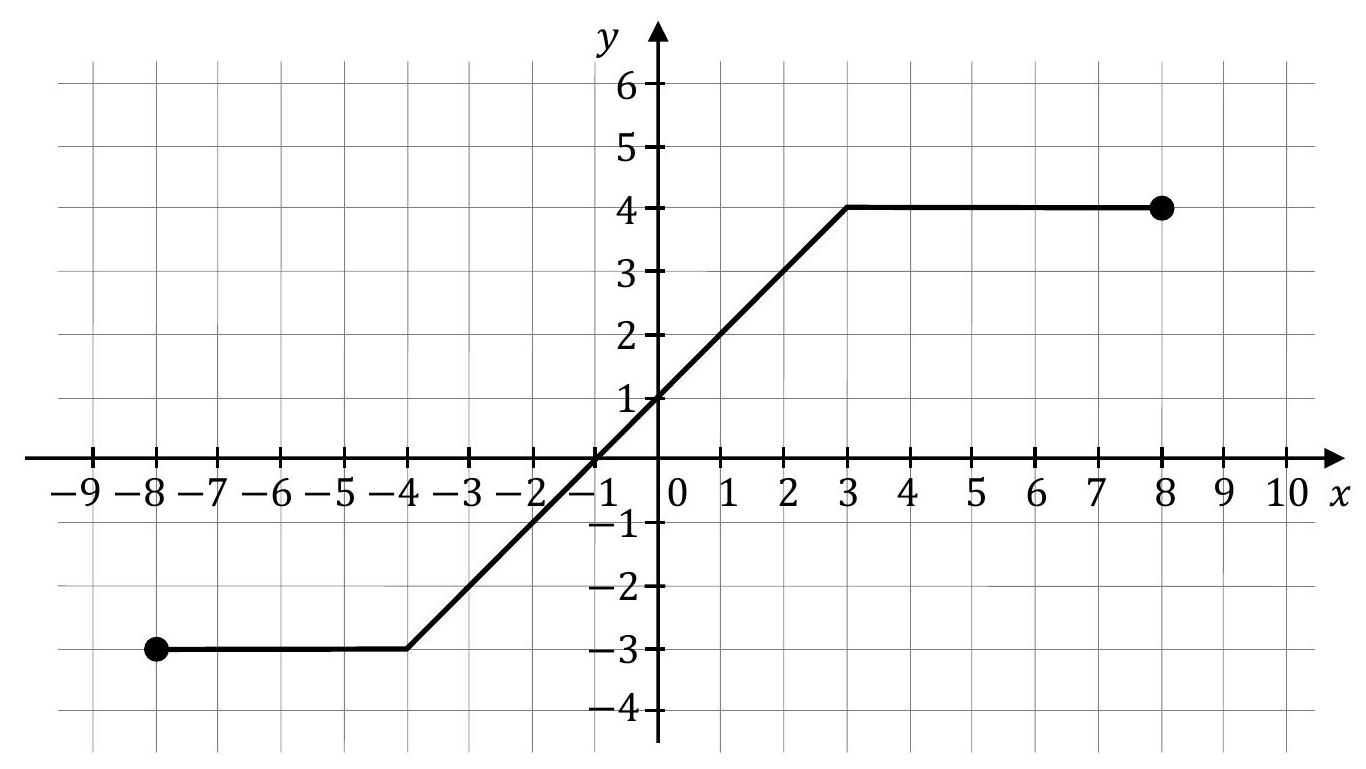
\includegraphics[max width=\textwidth, center]{2024_11_21_465acd0c12fa3e05e8a7g-04}\\
lloczyn \(f(-3) \cdot f(0) \cdot f(4)\) jest równy\\
A. \((-12)\)\\
B. \((-8)\)\\
C. 0\\
D. 16

BRUDNOPIS (nie podlega ocenie)\\

\includegraphics[max width=\textwidth, center]{2024_11_21_465acd0c12fa3e05e8a7g-05}

Zadanie 10. (0-1)\\
Na rysunku 1. przedstawiono wykres funkcji \(f\) określonej na zbiorze \(\langle-4,5\rangle\).

Rysunek 1.\\
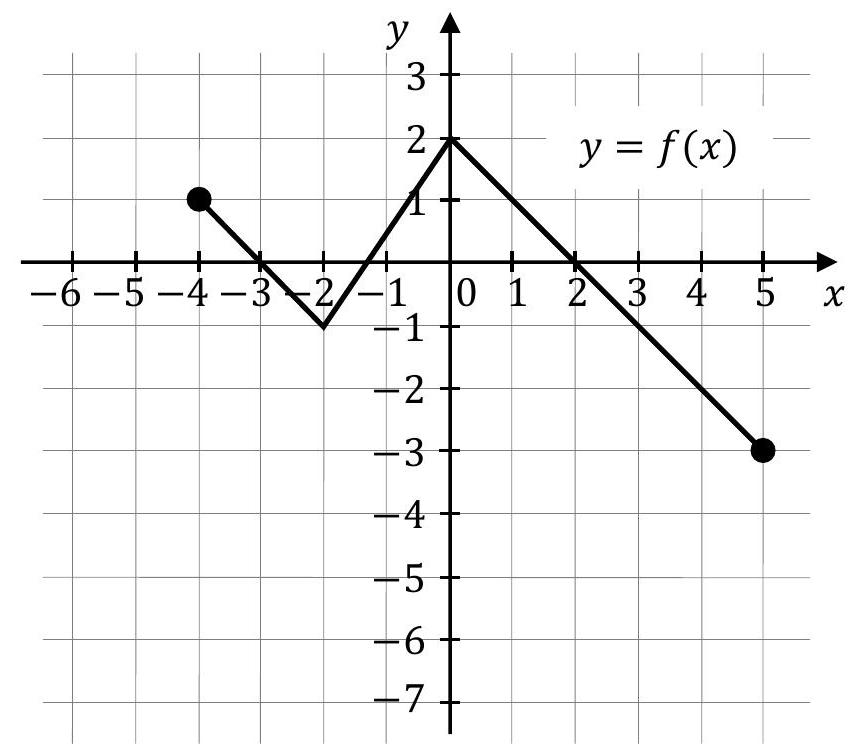
\includegraphics[max width=\textwidth, center]{2024_11_21_465acd0c12fa3e05e8a7g-06}

Funkcję \(g\) określono za pomocą funkcji \(f\). Wykres funkcji \(g\) przedstawiono na rysunku 2.

Rysunek 2.\\
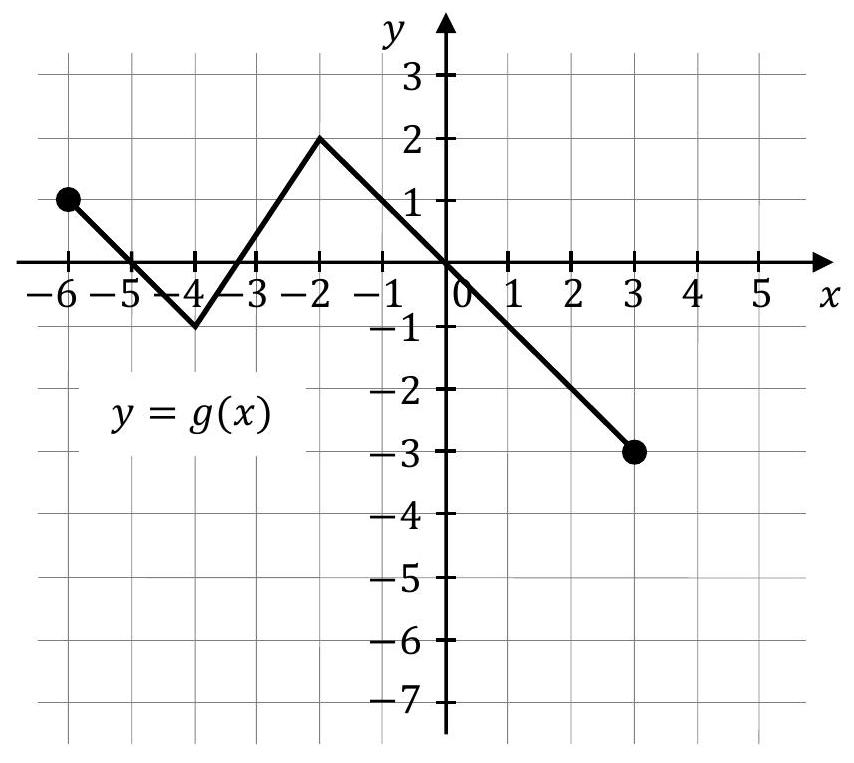
\includegraphics[max width=\textwidth, center]{2024_11_21_465acd0c12fa3e05e8a7g-06(1)}

Wynika stąd, że\\
A. \(g(x)=f(x)-2\)\\
B. \(g(x)=f(x-2)\)\\
C. \(g(x)=f(x)+2\)\\
D. \(g(x)=f(x+2)\)

\section*{BRUDNOPIS (nie podlega ocenie)}
\begin{center}

\includegraphics[max width=\textwidth]{2024_11_21_465acd0c12fa3e05e8a7g-07}
\end{center}

\section*{Zadanie 11. (0-1)}
Miejscem zerowym funkcji liniowej \(f\) określonej wzorem \(f(x)=-\frac{1}{3}(x+3)+5\) jest liczba\\
A. \((-3)\)\\
B. \(\frac{9}{2}\)\\
C. 5\\
D. 12

\section*{Zadanie 12. (0-1)}
Wykresem funkcji kwadratowej \(f(x)=3 x^{2}+b x+c\) jest parabola o wierzchołku w punkcie \(W=(-3,2)\). Wzór tej funkcji w postaci kanonicznej to\\
A. \(f(x)=3(x-3)^{2}+2\)\\
B. \(f(x)=3(x+3)^{2}+2\)\\
C. \(f(x)=(x-3)^{2}+2\)\\
D. \(f(x)=(x+3)^{2}+2\)

\section*{Zadanie 13. (0-1)}
Ciąg \(\left(a_{n}\right)\) jest określony wzorem \(a_{n}=\frac{2 n^{2}-30 n}{n}\) dla każdej liczby naturalnej \(n \geq 1\). Wtedy \(a_{7}\) jest równy\\
A. \((-196)\)\\
B. \((-32)\)\\
C. \((-26)\)\\
D. \((-16)\)

\section*{Zadanie 14. (0-1)}
W ciągu arytmetycznym \(\left(a_{n}\right)\), określonym dla każdej liczby naturalnej \(n \geq 1\), \(a_{5}=-31\) oraz \(a_{10}=-66\). Różnica tego ciągu jest równa\\
A. \((-7)\)\\
B. \((-19,4)\)\\
C. 7\\
D. 19,4

\section*{Zadanie 15. (0-1)}
Wszystkie wyrazy nieskończonego ciągu geometrycznego \(\left(a_{n}\right)\), określonego dla każdej liczby naturalnej \(n \geq 1\), są dodatnie i \(9 a_{5}=4 a_{3}\). Wtedy iloraz tego ciągu jest równy\\
A. \(\frac{2}{3}\)\\
B. \(\frac{3}{2}\)\\
C. \(\frac{2}{9}\)\\
D. \(\frac{9}{2}\)

\section*{Zadanie 16. (0-1)}
Liczba \(\cos 12^{\circ} \cdot \sin 78^{\circ}+\sin 12^{\circ} \cdot \cos 78^{\circ}\) jest równa\\
A. \(\frac{1}{2}\)\\
B. \(\frac{\sqrt{2}}{2}\)\\
C. \(\frac{\sqrt{3}}{2}\)\\
D. 1

BRUDNOPIS (nie podlega ocenie)\\

\includegraphics[max width=\textwidth, center]{2024_11_21_465acd0c12fa3e05e8a7g-09}

Zadanie 17. (0-1)\\
Punkty \(A, B, C\) leżą na okręgu o środku \(S\). Punkt \(D\) jest punktem przecięcia cięciwy \(A C\) i średnicy okręgu poprowadzonej z punktu \(B\). Miara kąta \(B S C\) jest równa \(\alpha\), a miara kąta \(A D B\) jest równa \(\gamma\) (zobacz rysunek).\\
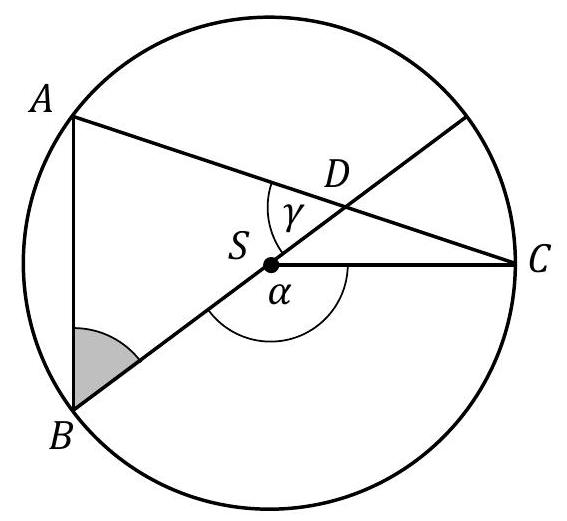
\includegraphics[max width=\textwidth, center]{2024_11_21_465acd0c12fa3e05e8a7g-10(1)}

Wtedy kąt \(A B D\) ma miarę\\
A. \(\frac{\alpha}{2}+\gamma-180^{\circ}\)\\
B. \(180^{\circ}-\frac{\alpha}{2}-\gamma\)\\
C. \(180^{\circ}-\alpha-\gamma\)\\
D. \(\alpha+\gamma-180^{\circ}\)

\section*{Zadanie 18. (0-1)}
Punkty \(A, B, P\) leżą na okręgu o środku \(S\) i promieniu 6. Czworokąt \(A S B P\) jest rombem, w którym kąt ostry \(P A S\) ma miarę \(60^{\circ}\) (zobacz rysunek).\\
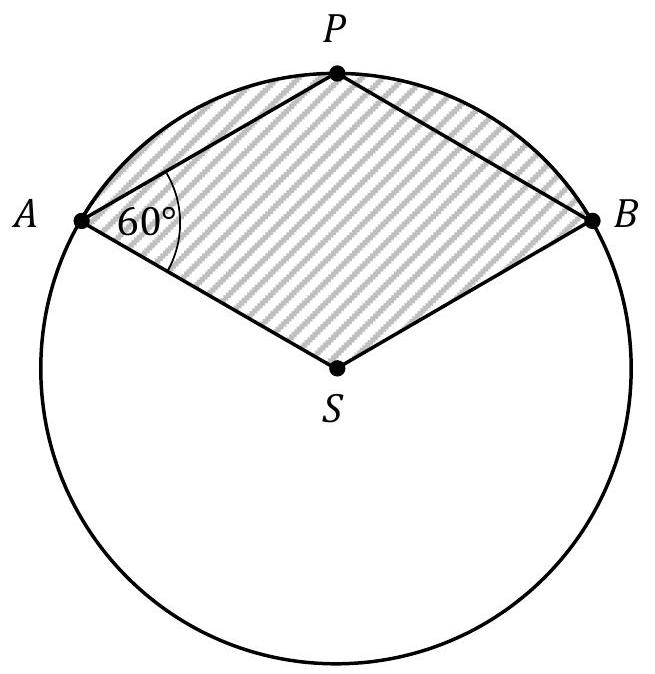
\includegraphics[max width=\textwidth, center]{2024_11_21_465acd0c12fa3e05e8a7g-10}

Pole zakreskowanej na rysunku figury jest równe\\
A. \(6 \pi\)\\
B. \(9 \pi\)\\
C. \(10 \pi\)\\
D. \(12 \pi\)

BRUDNOPIS (nie podlega ocenie)\\

\includegraphics[max width=\textwidth, center]{2024_11_21_465acd0c12fa3e05e8a7g-11}

Wysokość trójkąta równobocznego jest równa \(6 \sqrt{3}\). Pole tego trójkąta jest równe\\
A. \(3 \sqrt{3}\)\\
B. \(4 \sqrt{3}\)\\
C. \(27 \sqrt{3}\)\\
D. \(36 \sqrt{3}\)

\section*{Zadanie 20. (0-1)}
Boki równoległoboku mają długości 6 i 10, a kąt rozwarty między tymi bokami ma miarę \(120^{\circ}\). Pole tego równoległoboku jest równe\\
A. \(30 \sqrt{3}\)\\
B. 30\\
C. \(60 \sqrt{3}\)\\
D. 60

\section*{Zadanie 21. (0-1)}
Punkty \(A=(-2,6)\) oraz \(B=(3, b)\) leżą na prostej, która przechodzi przez początek układu współzędnych. Wtedy \(b\) jest równe\\
A. 9\\
B. \((-9)\)\\
C. \((-4)\)\\
D. 4

\section*{Zadanie 22. (0-1)}
Dane są cztery proste \(k, l, m, n\) o równaniach:\\
\(k: y=-x+1\)\\
\(l: y=\frac{2}{3} x+1\)\\
\(m: y=-\frac{3}{2} x+4\)\\
\(n: y=-\frac{2}{3} x-1\)

Wśród tych prostych prostopadłe sa\\
A. proste \(k\) oraz \(l\).\\
B. proste \(k\) oraz \(n\).\\
C. proste \(l\) oraz \(m\).\\
D. proste \(m\) oraz \(n\).

\section*{Zadanie 23. (0-1)}
Punkty \(K=(4,-10)\) i \(L=(b, 2)\) są końcami odcinka \(K L\). Pierwsza współzędna środka odcinka \(K L\) jest równa ( -12 ). Wynika stąd, że\\
A. \(b=-28\)\\
B. \(b=-14\)\\
C. \(b=-24\)\\
D. \(b=-10\)

BRUDNOPIS (nie podlega ocenie)\\

\includegraphics[max width=\textwidth, center]{2024_11_21_465acd0c12fa3e05e8a7g-13}

Zadanie 24. (0-1)\\
Punkty \(A=(-4,4)\) i \(B=(4,0)\) są sąsiednimi wierzchołkami kwadratu \(A B C D\). Przekątna tego kwadratu ma długość\\
A. \(4 \sqrt{10}\)\\
B. \(4 \sqrt{2}\)\\
C. \(4 \sqrt{5}\)\\
D. \(4 \sqrt{7}\)

\section*{Zadanie 25. (0-1)}
Podstawą graniastosłupa prostego jest romb o przekątnych długości 7 cm i 10 cm .\\
Wysokość tego graniastosłupa jest krótsza od dłuższej przekątnej rombu o 2 cm . Wtedy objętość graniastosłupa jest równa\\
A. \(560 \mathrm{~cm}^{3}\)\\
B. \(280 \mathrm{~cm}^{3}\)\\
C. \(\frac{280}{3} \mathrm{~cm}^{3}\)\\
D. \(\frac{560}{3} \mathrm{~cm}^{3}\)

\section*{Zadanie 26. (0-1)}
Dany jest sześcian \(A B C D E F G H\) o krawędzi długości \(a\). Punkty \(E, F, G, B\) są wierzchołkami ostrosłupa \(E F G B\) (zobacz rysunek).\\
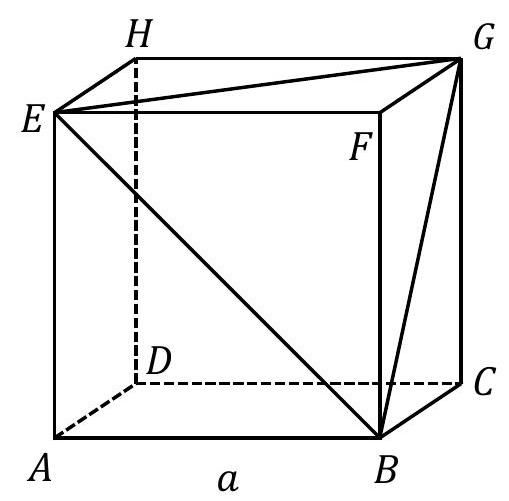
\includegraphics[max width=\textwidth, center]{2024_11_21_465acd0c12fa3e05e8a7g-14}

Pole powierzchni całkowitej ostrosłupa \(E F G B\) jest równe\\
A. \(a^{2}\)\\
B. \(\frac{3 \sqrt{3}}{2} \cdot a^{2}\)\\
C. \(\frac{3}{2} a^{2}\)\\
D. \(\frac{3+\sqrt{3}}{2} \cdot a^{2}\)

\section*{Zadanie 27. (0-1)}
Wszystkich różnych liczb naturalnych czterocyfrowych nieparzystych podzielnych przez 5 jest\\
A. \(9 \cdot 8 \cdot 7 \cdot 2\)\\
B. \(9 \cdot 10 \cdot 10 \cdot 1\)\\
C. \(9 \cdot 10 \cdot 10 \cdot 2\)\\
D. \(9 \cdot 9 \cdot 8 \cdot 1\)

\section*{Zadanie 28. (0-1)}
Średnia arytmetyczna zestawu sześciu liczb: \(2 x, 4,6,8,11,13\), jest równa 5 . Wynika stąd, że\\
A. \(x=-1\)\\
B. \(x=7\)\\
C. \(x=-6\)\\
D. \(x=6\)

BRUDNOPIS (nie podlega ocenie)\\

\includegraphics[max width=\textwidth, center]{2024_11_21_465acd0c12fa3e05e8a7g-15}

Zadanie 29. (0-2)\\
Rozwiąż nierówność:

\[
3 x^{2}-2 x-9 \geq 7
\]

\begin{center}
\begin{tabular}{|c|c|c|c|c|c|c|c|c|c|c|c|c|c|c|c|c|c|c|c|c|c|c|c|}
\hline
 &  &  &  &  &  &  &  &  &  &  &  &  &  &  &  &  &  &  &  &  &  &  &  \\
\hline
 &  &  &  &  &  &  &  &  &  &  &  &  &  &  &  &  &  &  &  &  &  &  &  \\
\hline
 &  &  &  &  &  &  &  &  &  &  &  &  &  &  &  &  &  &  &  &  &  &  &  \\
\hline
 &  &  &  &  &  &  &  &  &  &  &  &  &  &  &  &  &  &  &  &  &  &  &  \\
\hline
 &  &  &  &  &  &  &  &  &  &  &  &  &  &  &  &  &  &  &  &  &  &  &  \\
\hline
 &  &  &  &  &  &  &  &  &  &  &  &  &  &  &  &  &  &  &  &  &  &  &  \\
\hline
 &  &  &  &  &  &  &  &  &  &  &  &  &  &  &  &  &  &  &  &  &  &  &  \\
\hline
 &  &  &  &  &  &  &  &  &  &  &  &  &  &  &  &  &  &  &  &  &  &  &  \\
\hline
 &  &  &  &  &  &  &  &  &  &  &  &  &  &  &  &  &  &  &  &  &  &  &  \\
\hline
 &  &  &  &  &  &  &  &  &  &  &  &  &  &  &  &  &  &  &  &  &  &  &  \\
\hline
 &  &  &  &  &  &  &  &  &  &  &  &  &  &  &  &  &  &  &  &  &  &  &  \\
\hline
 &  &  &  &  &  &  &  &  &  &  &  &  &  &  &  &  &  &  &  &  &  &  &  \\
\hline
 &  &  &  &  &  &  &  &  &  &  &  &  &  &  &  &  &  &  &  &  &  &  &  \\
\hline
 &  &  &  &  &  &  &  &  &  &  &  &  &  &  &  &  &  &  &  &  &  &  &  \\
\hline
 &  &  &  &  &  &  &  &  &  &  &  &  &  &  &  &  &  &  &  &  &  &  &  \\
\hline
 &  &  &  &  &  &  &  &  &  &  &  &  &  &  &  &  &  &  &  &  &  &  &  \\
\hline
 &  &  &  &  &  &  &  &  &  &  &  &  &  &  &  &  &  &  &  &  &  &  &  \\
\hline
 &  &  &  &  &  &  &  &  &  &  &  &  &  &  &  &  &  &  &  &  &  &  &  \\
\hline
 &  &  &  &  &  &  &  &  &  &  &  &  &  &  &  &  &  &  &  &  &  &  &  \\
\hline
 &  &  &  &  &  &  &  &  &  &  &  &  &  &  &  &  &  &  &  &  &  &  &  \\
\hline
 &  &  &  &  &  &  &  &  &  &  &  &  &  &  &  &  &  &  &  &  &  &  &  \\
\hline
 &  &  &  &  &  &  &  &  &  &  &  &  &  &  &  &  &  &  &  &  &  &  &  \\
\hline
 &  &  &  &  &  &  &  &  &  &  &  &  &  &  &  &  &  &  &  &  &  &  &  \\
\hline
 &  &  &  &  &  &  &  &  &  &  &  &  &  &  &  &  &  &  &  &  &  &  &  \\
\hline
 &  &  &  &  &  &  &  &  &  &  &  &  &  &  &  &  &  &  &  &  &  &  &  \\
\hline
 &  &  &  &  &  &  &  &  &  &  &  &  &  &  &  &  &  &  &  &  &  &  &  \\
\hline
 &  &  &  &  &  &  &  &  &  &  &  &  &  &  &  &  &  &  &  &  &  &  &  \\
\hline
 &  &  &  &  &  &  &  &  &  &  &  &  &  &  &  &  &  &  &  &  &  &  &  \\
\hline
 &  &  &  &  &  &  &  &  &  &  &  &  &  &  &  &  &  &  &  &  &  &  &  \\
\hline
 &  &  &  &  &  &  &  &  &  &  &  &  &  &  &  &  &  &  &  &  &  &  &  \\
\hline
 &  &  &  &  &  &  &  &  &  &  &  &  &  &  &  &  &  &  &  &  &  &  &  \\
\hline
 &  &  &  &  &  &  &  &  &  &  &  &  &  &  &  &  &  &  &  &  &  &  &  \\
\hline
 &  &  &  &  &  &  &  &  &  &  &  &  &  &  &  &  &  &  &  &  &  &  &  \\
\hline
 &  &  &  &  &  &  &  &  &  &  &  &  &  &  &  &  &  &  &  &  &  &  &  \\
\hline
 &  &  &  &  &  &  &  &  &  &  &  &  &  &  &  &  &  &  &  &  &  &  &  \\
\hline
 &  &  &  &  &  &  &  &  &  &  &  &  &  &  &  &  &  &  &  &  &  &  &  \\
\hline
 &  &  &  &  &  &  &  &  &  &  &  &  &  &  &  &  &  &  &  &  &  &  &  \\
\hline
 &  &  &  &  &  &  &  &  &  &  &  &  &  &  &  &  &  &  &  &  &  &  &  \\
\hline
 &  &  &  &  &  &  &  &  &  &  &  &  &  &  &  &  &  &  &  &  &  &  &  \\
\hline
 &  &  &  &  &  &  &  &  &  &  &  &  &  &  &  &  &  &  &  &  &  &  &  \\
\hline
 &  &  &  &  &  &  &  &  &  &  &  &  &  &  &  &  &  &  &  &  &  &  &  \\
\hline
 &  &  &  &  &  &  &  &  &  &  &  &  &  &  &  &  &  &  &  &  &  &  &  \\
\hline
 &  &  &  &  &  &  &  &  &  &  &  &  &  &  & - &  & - & - & - & - &  &  &  \\
\hline
 &  &  &  &  &  &  &  &  &  &  &  &  &  &  &  &  &  &  &  &  &  &  &  \\
\hline
\end{tabular}
\end{center}

Zadanie 30. (0-2)\\
W ciągu arytmetycznym \(\left(a_{n}\right)\), określonym dla każdej liczby naturalnej \(n \geq 1\), \(a_{1}=-1\) i \(a_{4}=8\). Oblicz sumę stu początkowych kolejnych wyrazów tego ciągu.\\

\includegraphics[max width=\textwidth, center]{2024_11_21_465acd0c12fa3e05e8a7g-17}

\begin{center}
\begin{tabular}{|c|l|c|c|}
\hline
\multirow{2}{*}{\begin{tabular}{c}
Wypełnia \\
egzaminator \\
\end{tabular}} & Nr zadania & 29. & 30. \\
\cline { 2 - 4 }
 & Maks. liczba pkt & 2 & 2 \\
\cline { 2 - 4 }
 & Uzyskana liczba pkt &  &  \\
\hline
\end{tabular}
\end{center}

Zadanie 31. (0-2)\\
Wykaż, że dla każdej liczby rzeczywistej \(a\) i każdej liczby rzeczywistej \(b\) takich, że \(b \neq a\), spełniona jest nierówność

\[
\frac{a^{2}+b^{2}}{2}>\left(\frac{a+b}{2}\right)^{2}
\]

\begin{center}

\includegraphics[max width=\textwidth]{2024_11_21_465acd0c12fa3e05e8a7g-18}
\end{center}

Zadanie 32. (0-2)\\
Kąt \(\alpha\) jest ostry i \(\operatorname{tg} \alpha=2\). Oblicz wartość wyrażenia \(\sin ^{2} \alpha\).\\

\includegraphics[max width=\textwidth, center]{2024_11_21_465acd0c12fa3e05e8a7g-19}

Wypełnia egzaminator

\begin{center}
\begin{tabular}{|l|c|c|}
\hline
Nr zadania & 31. & 32. \\
\hline
Maks. liczba pkt & 2 & 2 \\
\hline
Uzyskana liczba pkt &  &  \\
\hline
\end{tabular}
\end{center}

Zadanie 33. (0-2)\\
Dany jest trójkąt równoramienny \(A B C\), w którym \(|A C|=|B C|\). Dwusieczna kąta \(B A C\) przecina bok \(B C\) w takim punkcie \(D\), że trójkąty \(A B C\) i \(B D A\) są podobne (zobacz rysunek). Oblicz miarę kąta \(B A C\).\\

\includegraphics[max width=\textwidth, center]{2024_11_21_465acd0c12fa3e05e8a7g-20}

Zadanie 34. (0-2)\\
Ze zbioru dziewięcioelementowego \(M=\{1,2,3,4,5,6,7,8,9\}\) losujemy kolejno ze zwracaniem dwa razy po jednej liczbie. Zdarzenie \(A\) polega na wylosowaniu dwóch liczb ze zbioru \(M\), których iloczyn jest równy 24. Oblicz prawdopodobieństwo zdarzenia \(A\).\\

\includegraphics[max width=\textwidth, center]{2024_11_21_465acd0c12fa3e05e8a7g-21}

\begin{center}
\begin{tabular}{|c|l|c|c|}
\hline
\multirow{2}{*}{\begin{tabular}{c}
Wypełnia \\
egzaminator \\
\end{tabular}} & Nr zadania & 33. & 34. \\
\cline { 2 - 4 }
 & Maks. liczba pkt & 2 & 2 \\
\cline { 2 - 4 }
 & Uzyskana liczba pkt &  &  \\
\hline
\end{tabular}
\end{center}

Zadanie 35. (0-5)\\
Wykres funkcji kwadratowej \(f\) określonej wzorem \(f(x)=a x^{2}+b x+c\) ma z prostą o równaniu \(y=6\) dokładnie jeden punkt wspólny. Punkty \(A=(-5,0)\) i \(B=(3,0)\) należą do wykresu funkcji \(f\). Oblicz wartości współczynników \(a, b\) oraz \(c\).\\

\includegraphics[max width=\textwidth, center]{2024_11_21_465acd0c12fa3e05e8a7g-22}\\

\includegraphics[max width=\textwidth, center]{2024_11_21_465acd0c12fa3e05e8a7g-23}

\begin{center}
\begin{tabular}{|c|l|c|}
\hline
\multirow{3}{*}{\begin{tabular}{c}
Wypełnia \\
egzaminator \\
\end{tabular}} & Nr zadania & 35. \\
\cline { 2 - 3 }
 & Maks. liczba pkt & 5 \\
\cline { 2 - 3 }
 & Uzyskana liczba pkt &  \\
\hline
\end{tabular}
\end{center}

BRUDNOPIS (nie podlega ocenie)\\

\includegraphics[max width=\textwidth, center]{2024_11_21_465acd0c12fa3e05e8a7g-24}\\

\includegraphics[max width=\textwidth, center]{2024_11_21_465acd0c12fa3e05e8a7g-25}


\end{document}